\documentclass[12pt,a4paper]{report}

%
% PACKAGES AND STYLES
%

% 
% Language and encoding
%
%\usepackage{mathtext}
%\usepackage[T2A]{fontenc}
\usepackage[utf8]{inputenc}
\usepackage[english,russian]{babel}
\usepackage{mmap}

%
% Colors
%
\usepackage[usenames]{color}
\usepackage{color}
\usepackage{colortbl}

%
% Symbols
%
\usepackage{amssymb}
\usepackage{MnSymbol}

%
% Units
%
%\usepackage[binary-units=true]{siunitx}
\newcommand{\km}{\mathrm{~\text{км}}}
\newcommand{\m}{\mathrm{~\text{м}}}
\newcommand{\s}{\mathrm{~\text{с}}}
\newcommand{\mps}{\m \s ^{-1}}
\newcommand{\pers}{\s ^{-1}}
\newcommand{\K}{\mathrm{~\text{К}}}
\newcommand{\Kpkm}{\K\km ^{-1}}
\newcommand{\hpa}{\mathrm{~\text{гПа}}}
\newcommand{\J}{\mathrm{~\text{Дж}}}
\newcommand{\Jpm}{\J \m ^{-3}}

%
% Paper size and margins
%
\usepackage{vmargin}
\setmarginsrb{2.5cm}{1cm}{2.5cm}{2cm}{0cm}{0cm}{0cm}{1.5cm}

%
% Page style
%
\usepackage{fancyhdr}
\setlength{\headheight}{16pt}
\newcommand{\changefont}{%
    \fontsize{9}{11}\selectfont
}
\fancyhf{}
\fancyhead[RO]{\changefont \slshape \rightmark} %section
\fancyhead[LO]{\changefont \slshape \leftmark} %chapter
\fancyfoot[C]{\changefont \thepage} %footer
\setlength{\headsep}{0.2in}
\pagestyle{fancy}

%
% Indenting
%
\usepackage{indentfirst}
\setlength{\parindent}{1cm}
\setlength{\parskip}{0.5cm}

%
% References
%
\usepackage{natbib}

%
% Hyperlinks
%
\usepackage[linktocpage=true,plainpages=false,pdfpagelabels=false]{hyperref}
\definecolor{linkcolor}{rgb}{0.1,0,0.9}
\definecolor{citecolor}{rgb}{0,0,0.9}
\definecolor{urlcolor}{rgb}{0,0,1}
\hypersetup{
    colorlinks, linkcolor={linkcolor},
    citecolor={citecolor}, urlcolor={urlcolor}
}

\bibliographystyle{plainnat}
% Bibliography: set article volume number in bold font
%\DeclareFieldFormat
%  [article]
%  {volume}{\textbf{#1}}
%\renewcommand\nameyeardelim{, }

%\usepackage{showkeys} % show labels

\newcommand{\figref}[1]{\mbox{Figure~\ref{#1}}}
\newcommand{\tabref}[1]{\mbox{Table~\ref{#1}}}
\newcommand{\secref}[1]{\mbox{Section~\ref{#1}}}
\newcommand{\chpref}[1]{\mbox{Chapter~\ref{#1}}}
\newcommand{\appref}[1]{\mbox{Appendix~\ref{#1}}}
\newcommand{\eqnref}[1]{\mbox{Eq.~(\ref{#1})}}
\newcommand{\listref}[1]{\mbox{Listing~(\ref{#1})}}

%
% Lists
%
\usepackage[shortlabels]{enumitem}

\newenvironment{sqlist}[1][\enskip$\filledsquare$]
        {\begin{itemize}[#1]}
        {\end{itemize}}

% New math commands
% differential d, from http://tex.stackexchange.com/a/60546/586
\newcommand*\diff{\mathop{}\!\mathrm{d}}
\newcommand\mean[1]{\overline{#1}}
\newcommand{\PDt}[2]{\partial #1/\partial #2}

%
% Tables
%
\usepackage{booktabs}
%\usepackage{tabularx}
\usepackage{tabu}
\usepackage{longtable}

%
% Figures
%
\usepackage{wrapfig}
\usepackage[font=small,textfont=it,labelfont=bf]{caption}
%\captionsetup[figure]{labelfont=bf}
\usepackage{tikz}
\usepackage{pgfplots}
\usetikzlibrary{calc}

%
% Equations
%
\usepackage{cool}


\begin{document}
\setcounter{chapter}{2}
\chapter{Численные эксперименты}
\label{ch:experiments}
\section{Мезомасштабная модель ReMeDy}
Оригинальная версия модели \citep{MillerWhite1984,XueThorpe1991} основана на двумерном представлении прогностических уравнений с использованием $\sigma$-координаты; в дальнейшем наряду с модификацией граничных условий и включением эффектов вращения была преобразована в трехмерную \citep{MirandaPhD}. Данная модель использовалась при исследовании ледового бриза \citep{ChechinEtAl2013} и в настоящее время развивается в Научно-исследовательском вычислительном центре МГУ. Современное состояние модели изложено в виде табл. \ref{tab:model}

\renewcommand{\arraystretch}{2}
\begin{table}
\centering
\caption{Характеристики модели ReMeDy}
\label{tab:model}
\small
\begin{tabu} to \textwidth {p{5cm}X[l]}
\toprule
Система уравнений & Негидростатическая, трехмерная \\
Учет силы Кориолиса & Приближение $f$-плоскости \\
Радиация & Блок переноса коротковолновой и длинноволновой радиации CLIRAD-SW и CLIRAD-LW (ссылки в \citep{StepanenkoMikushin2008})\\
Примеси & Блок переноса атмосферной примеси \citep{StepanenkoMikushin2008} \\
Турбулентное замыкание	& Локальное замыкание Смагоринского-Лилли \citep{Smagorinsky1958,Lilly1962}, нелокальное замыкание Люпкеса-Шлюнцен \citep{LupkesSchluenzen1996,NohEtAl2003} \\
Подстилающая поверхность & Модель деятельного слоя ИВМ РАН \citep{VolodinLykosov1998} \\
Параметризация водоемов (поверхностного слоя океана)	& Одномерная модель водоема LAKE \citep{StepanenkoEtAl2011} \\
Фазовые переходы воды & Параметризация микрофизики облаков и осадков при положительной температуре \citep{TeixeiraMiranda1997}\\
Вертикальная координата & $\sigma=\frac{p-p_{top}}{p_*}$, где $p_*=p_{surf}-p_{top}$, $p_{surf}$ -- давление на земной поверхности, $p_{top}$ -- давление на верхней границе расчетной области \\
Боковые граничные условия & Периодические, однородные Неймана, Дирихле, излучения \\
Верхнее и нижнее граничные условия & Однородное условие Неймана для горизонтальных составляющих скорости, условия Дирихле для вертикальной скорости; для температуры и примесей задаются потоки на поверхности \\
Рэлеевское трение в буферной зоне & Применяется к сеточному решению вблизи верхней и горизонтальных границ области. Это позволяет частично подавить схемные возмущения, возникающие около границ. С помощью тригонометрической функции обеспечивается притяжение метеорологических полей к значениям на внутренней границе буферной зоны или к фоновому состоянию. \\
Дискретизация производных & По пространству: схема центральных разностей, по времени: явная схема второго порядка 'чехарда' \\
Численная фильтрация & Пространственный фильтр 4-го порядка для подавления волн (максимально – с длиной в два шага сетки), фильтр Аселина для подавления временной вычислительной моды \\
Пространственная сетка & $C$-сетка Аракавы (см. \ref{sec:model:grid})\\
\bottomrule
\end{tabu}
\end{table}

\subsection{Система уравнений}
Вывод системы уравнений модели представлен в \ref{app:A}. Чтобы улучшить свойства численного решения, прогностические уравнения модели написаны в потоковой форме. Это позволяет представить адвективные слагаемые в форме дивергенции соответствующего вектора потока. После интегрирования по расчетной области, вклад этих слагаемых проявляется через граничные условия, что исключает ложную генерацию энергии в пределах этой области и тем самым позволяет контролировать нелинейную неустойчивость. Полная система прогностических уравнений в потоковой форме выглядят так:
\begin{subequations}\label{eq:progn0}
\begin{align}
\frac{\partial{up_*}}{\partial{t}} + \frac{\partial{u^2p_*}}{\partial{x}}+ \frac{\partial{vup_*}}{\partial{y}}+ \frac{\partial{\dot{\sigma}up_*}}{\partial{\sigma}}&=-p_* \frac{\partial{\phi'}}{\partial{x}}+\sigma \frac{\partial{p_*}}{\partial{x}}\frac{\partial{\phi'}}{\partial{\sigma}}+f(v-V_g )p_*+p_*(D_u+R_u )\label{eq:progn1} \\
\frac{\partial{vp_*}}{\partial{t}} + \frac{\partial{uv^2p_*}}{\partial{x}}+ \frac{\partial{v^2p_*}}{\partial{y}}+ \frac{\partial{\dot{\sigma}vp_*}}{\partial{\sigma}}&=-p_* \frac{\partial{\phi'}}{\partial{y}}+\sigma \frac{\partial{p_*}}{\partial{y}}\frac{\partial{\phi'}}{\partial{\sigma}}-f(u-U_g )p_*+p_*(D_v+R_v )\label{eq:progn2} \\
\frac{\partial{\tilde{w}p_*}}{\partial{t}} + \frac{\partial{u\tilde{w}p_*}}{\partial{x}}+ \frac{\partial{v\tilde{w}p_*}}{\partial{y}}+ \frac{\partial{\dot{\sigma}\tilde{w}p_*}}{\partial{\sigma}}&=S_vp_*\frac{\partial{\phi'}}{\partial{\sigma}}+p_*g(\frac{\theta'}{\theta_S}-q_r)+p_*(D_{\tilde{w}}+R_{\tilde{w}})\label{eq:progn3} \\
\frac{\partial{\theta'p_*}}{\partial{t}} + \frac{\partial{u\theta'p_*}}{\partial{x}}+ \frac{\partial{v\theta'p_*}}{\partial{y}}+ \frac{\partial{\dot{\sigma}\theta'p_*}}{\partial{\sigma}}&=S_v\tilde{w}p_* \frac{\partial{\theta_s}}{\partial{\sigma}}+p_*Q+p_*(D_{\theta}+R_{\theta})\label{eq:progn4} \\
\frac{\partial{p_*}}{\partial{t}} + \frac{\partial{up_*}}{\partial{x}}+ \frac{\partial{vp_*}}{\partial{y}}+ \frac{\partial{\dot{\sigma}p_*}}{\partial{\sigma}}&=0\label{eq:progn5} \\
\frac{\partial{q_vp_*}}{\partial{t}} + \frac{\partial{uq_vp_*}}{\partial{x}}+ \frac{\partial{vq_vp_*}}{\partial{y}}+ \frac{\partial{\dot{\sigma}q_vp_*}}{\partial{\sigma}}&=p_*(E-C)+p_*(D_{q_v}+R_{q_v})\label{eq:progn6} \\
\frac{\partial{q_cp_*}}{\partial{t}} + \frac{\partial{uq_cp_*}}{\partial{x}}+ \frac{\partial{vq_cp_*}}{\partial{y}}+ \frac{\partial{\dot{\sigma}q_cp_*}}{\partial{\sigma}}&=p_*(C-A)+p_*(D_{q_c}+R_{q_c})\label{eq:progn7} \\
\frac{\partial{q_rp_*}}{\partial{t}} + \frac{\partial{uq_rp_*}}{\partial{x}}+ \frac{\partial{vq_rp_*}}{\partial{y}}+ \frac{\partial{\dot{\sigma}q_rp_*}}{\partial{\sigma}}&=p_*(A-E)-g\frac{\partial{\rho V_rq_r}}{\partial\sigma}+p_*(D_{q_r}+R_{q_r})\label{eq:progn8}
\end{align}
\end{subequations}
где $t$ --- время, $x$ --- горизонтальная координата, направленная на восток, $y$ --- горизонтальная координата, направленная на север, $\sigma$ --- вертикальная координата, $\sigma=\frac{p-p_{top}}{p_*}$, $p_*=p_{surf}-p_{top}$, $p$ --- атмосферное давление, $p_{surf}$ --- приземное давление, $p_{top}$ --- давление на верхней границе расчетной области, $u$ --- составляющая скорости вдоль оси $X$, $v$ - составляющая скорости вдоль оси $Y$, $\tilde{w}$ --- аппроксимация составляющей скорости вдоль $Z$, $\dot{\sigma}$ --- аналог вертикальной скорости в $\sigma$-координатах, $\phi'$ --- возмущение геопотенциала, $(U_g,V_g)$ --- вектор геострофического ветра, $f$ --- параметр Кориолиса, $\phi'$ --- отклонение геопотенциала, $\theta'$ --- отклонение потенциальной температуры, $S_v=\frac{gp}{R_dT_{vs}p_*}$, $Q=\frac{L_v}{c_p}\left(\frac{p_0}{p}\right)^{R_d/c_p}(C-E)$ --- неадиабатическое нагревание, $c_p$ --- удельная теплоемкость при постоянном давлении, $L_v$ --- удельная теплота конденсация, $p_0=1000\hpa$, $q_r$ --- удельное содержание дождевых капель, $q_v$ --- удельная влажность, $q_c$ --- удельное содержание облачных капель, $C$ --- скорость конденсации, $E$ --- скорость испарения, $A$ --- суммарная интенсивность захвата облачных капель осадками и автоконверсии, $V_r$ --- скорость падения дождевых капель, $D$ --- слагаемые, описывающие турбулентную диффузию соответствующих субстанций, $R$ --- дополнительные слагаемые, включающие, в частности, пространственные и временные фильтры в конечно-разностной схеме модели. Верхними штрихами обозначены отклонения величин от их фоновых значений. Фоновые значения зависят только от давления и обозначены нижним индексом $s$.

Для замыкания системы уравнений используется диагностическое уравнение для возмущения геопотенциала $\phi'$. оно может быть получено путем некоторых преобразований из уравнений движения и уравнения неразрывности. В полном виде это уравнение приводится в \citep{MirandaPhD}.

Входящие в последние три уравнения \eqref{eq:progn0} переходы атмосферной влаги из одного фазового состояния в другое описываются с помощью параметризаций микрофизических процессов. Для параметризации облачной микрофизики без учета твердой фазы используется схема Кесслера, а соответствующие модификации, включенные в модель ReMeDy, описаны в отчете \citep{TeixeiraMiranda1997}.

\subsection{Конечно-разностная сетка модели}
\label{sec:model:grid}
Дискретизация системы уравнений проводится на разнесеннной C-сетке Аракавы (рис. \ref{fig:modelgrid}), так что пространственные производные аппроксимируются центральными разностями второго порядка точности. Интегрирование уравнений по времени проводится по явной схеме второго порядка точности, называемой схемой «чехарда».
$$x_i=(i-3/2)\Delta x,i=1,N_x+1$$
$$y_i=(i-3/2)\Delta x,i=1,N_y+1$$
$$\sigma: \sigma_0, \dots, \sigma_k,\dots,\sigma_{N_s},$$
где $N_x$, $N_y$ – число узлов в направлениях $x,y$ горизонтальной плоскости, $N_s$ – число вертикальных уровней по координате $\sigma$. Уравнения модели записаны для постоянного шага сетки в обоих горизонтальных направлениях, и в рассматриваемых экспериментах принимается их равенство. Что касается разрешения по вертикальной координате, то оно является переменным, благодаря чему достигается повышенная детализация процессов в пограничном слое. 
Решение уравнений проводится только для внутренних точек области интегрирования, а значения переменных в точках на границах и за ними (вследствие разнесения переменных на шаблоне схемы) получаются из граничных условий.
\begin{figure}[h]
\begin{center}
\begin{tikzpicture}
	%%% Edit the following coordinate to change the shape of your
	%%% cuboid
      
	%% Vanishing points for perspective handling
	\coordinate (P1) at (-15cm,5cm); % left vanishing point (To pick)
	\coordinate (P2) at (15cm,5cm); % right vanishing point (To pick)

	%% (A1) and (A2) defines the 2 central points of the cuboid
	\coordinate (A1) at (0em,0cm); % central top point (To pick)
	\coordinate (A2) at (0em,-4cm); % central bottom point (To pick)

	%% (A3) to (A8) are computed given a unique parameter (or 2) .8
	% You can vary .8 from 0 to 1 to change perspective on left side
	\coordinate (A3) at ($(P1)!.8!(A2)$); % To pick for perspective 
	\coordinate (A4) at ($(P1)!.8!(A1)$);

	% You can vary .8 from 0 to 1 to change perspective on right side
	\coordinate (A7) at ($(P2)!.7!(A2)$);
	\coordinate (A8) at ($(P2)!.7!(A1)$);

	%% Automatically compute the last 2 points with intersections
	\coordinate (A5) at
	  (intersection cs: first line={(A8) -- (P1)},
			    second line={(A4) -- (P2)});
	\coordinate (A6) at
	  (intersection cs: first line={(A7) -- (P1)}, 
			    second line={(A3) -- (P2)});

	%%% Depending of what you want to display, you can comment/edit
	%%% the following lines

	%% Possibly draw back faces
%
%	\fill[gray!90] (A2) -- (A3) -- (A6) -- (A7) -- cycle; % face 6
%	\node at (barycentric cs:A2=1,A3=1,A6=1,A7=1) {\tiny f6};
%	
%	\fill[gray!50] (A3) -- (A4) -- (A5) -- (A6) -- cycle; % face 3
%	\node at (barycentric cs:A3=1,A4=1,A5=1,A6=1) {\tiny f3};
%	
%	\fill[gray!30] (A5) -- (A6) -- (A7) -- (A8) -- cycle; % face 4
%	\node at (barycentric cs:A5=1,A6=1,A7=1,A8=1) {\tiny f4};
	
	\draw[thick,dashed,gray] (A5) -- (A6);
	\draw[thick,dashed,gray] (A3) -- (A6);
	\draw[thick,dashed,gray] (A7) -- (A6);

	%% Possibly draw front faces

	% \fill[orange] (A1) -- (A8) -- (A7) -- (A2) -- cycle; % face 1
	% \node at (barycentric cs:A1=1,A8=1,A7=1,A2=1) {\tiny f1};
%	\fill[gray!50,opacity=0.2] (A1) -- (A2) -- (A3) -- (A4) -- cycle; % f2
%	\node at (barycentric cs:A1=1,A2=1,A3=1,A4=1) {\tiny f2};
%	\fill[gray!90,opacity=0.2] (A1) -- (A4) -- (A5) -- (A8) -- cycle; % f5
%	\node at (barycentric cs:A1=1,A4=1,A5=1,A8=1) {\tiny f5};

	%% Possibly draw front lines
	\draw[thick,gray] (A1) -- (A2);
	\draw[thick,gray] (A3) -- (A4);
	\draw[thick,gray] (A7) -- (A8);
	\draw[thick,gray] (A1) -- (A4);
	\draw[thick,gray] (A1) -- (A8);
	\draw[thick,gray] (A2) -- (A3);
	\draw[thick,gray] (A2) -- (A7);
	\draw[thick,gray] (A4) -- (A5);
	\draw[thick,gray] (A8) -- (A5);
	
	% Possibly draw points
	% (it can help you understand the cuboid structure)
%	\foreach \i in {1,2,...,8}
%	{
%	\draw[fill=black] (A\i) circle (0.1em) node[above] {\small \i};
%	}
	  \draw[fill=gray] (A1) circle (0.15em) node[text width=1cm, below left] {\small $\dot{\sigma},\tilde{w}$ \\ $\mathcal{F}_w,\mathcal{D}_w$};
	  \draw[fill=gray] (A1) circle (0.15em) node[text width=1cm, above left] {\small $(x_{i},y_{j},\sigma_{k-1/2})$ \\  \quad};
	  
	  \draw[fill=gray] (A2) circle (0.15em) node[text width=1cm,left] {\small $\theta,\phi,p_*$ \\ $Def, Ri$};
	  \draw[fill=gray] (A2) circle (0.15em) node[text width=1cm,below] {\small \\$(x_{i},y_{j},\sigma_{k})$};
	  
	  \draw[fill=gray] (A7) circle (0.15em) node[text width=1cm,above right] {\small $u$ \\ $\mathcal{F}_u,\mathcal{D}_u$};
	  \draw[fill=gray] (A7) circle (0.15em) node[text width=1cm,below right] {\small \\$(x_{i+1/2},y_{j},\sigma_{k})$};
	  
	  \draw[fill=gray] (A3) circle (0.15em) node[text width=1cm,above left] {\small $v$ \\ $\mathcal{F}_v,\mathcal{D}_v$};
	  \draw[fill=gray] (A3) circle (0.15em) node[text width=1cm,right] {\small \\$(x_{i},y_{j+1/2},\sigma_{k})$};

	% \draw[fill=black] (P1) circle (0.1em) node[below] {\tiny p1};
	% \draw[fill=black] (P2) circle (0.1em) node[below] {\tiny p2};
\end{tikzpicture}
\end{center}
\caption{Модельная $C$-сетка Аракавы}
\label{fig:modelgrid}
\end{figure}

В настоящее время модель ReMeDy имеет параллельную реализацию по технологии MPI \citep{StepanenkoMikushin2008}. Благодаря этому, время счета каждого экспериментов составляло в среднем около 2 часов при запуске на 16 процессорах суперкомпьютерного кластера МГУ 'Ломоносов' \citep{VoevodinEtAl2012}.

\subsection{Параметризация подсеточного перемешивания}
\label{sec:model:closure}
\subsubsection{Локальное замыкание}
Для параметризации турбулентных потоков над приземным слоем в оригинальной версии модели предполагалось использование локального замыкания турбулентности первого порядка, разработанного Смагоринским \citep{Smagorinsky1958} для крупномасштабного моделирования и затем дополненного Лилли \citep{Lilly1962}. В этой схеме подсеточное перемешивание учитывается путем включения в уравнения движения вязких слагаемых вида
\begin{equation}
D_i=\frac{1}{\rho}\pderiv{\tau_{ij}}{x_{j}}
\end{equation} 
и в уравнение для температуры слагаемого вида
\begin{equation} \label{eq:subgrid_flux}
D_\theta=\frac{1}{\rho}\pderiv{H_j}{x_j},
\end{equation}
где используется правило суммирования по повторяющимся индексам, т.е. $x_1=x, x_2=y, x_3=z$ --- три декартовы координаты, $D_1=D_u, D_2=D_v, D_3=D_w$. Тензор напряжений определяется пропорционально тензору деформаций:
\begin{equation}
\tau_{ij}=\rho K_M \mathsf{D}_{ij},
\end{equation}
где тензор деформации зависит от пространственных производных скорости. Аналогичным образом определяется поток тепла в ур. \eqref{eq:subgrid_flux}:
\begin{equation}
H_j = \rho K_H \pderiv{\theta}{x_j}.
\end{equation}
Соотношение между коэффициентами турбулентного обмена теплом $K_H$ и импульсом $K_M$ также записывается в терминах тензора деформации:
\begin{equation}
K_M = (k\Delta)^2 Def\left[max\left(0,(1-\epsilon\frac{K_H}{K_M}Ri)\right)\right]^{0.5},
\end{equation}
где $\epsilon$ --- параметр, включающий зависимость $K_M$ от устойчивости; $\frac{K_H}{K_M}=\frac{1}{Pr}$, где $Pr$ --- число Прандтля; $k=0.21$ --- константа; $\Delta = min(\Delta x, \Delta y, \Delta z)$;
\begin{equation}
Def = \frac{1}{2}\left(\mathsf{D}_{11}^2 + \mathsf{D}_{22}^2 + \mathsf{D}_{33}^2 \right) + \mathsf{D}_{12}^2 + \mathsf{D}_{13}^2 + \mathsf{D}_{23}^2;
\end{equation}
$Ri$ --- число Ричардсона:
\begin{equation}
Ri = \frac{N^2}{Def^2} \approx -S\frac{g}{\theta}\pderiv{\theta}{\sigma}Def^{-2},
\end{equation}
где $N$ --- частота Брента-Вяйсяля.

Таким образом, в общей форме коэффициенты турбулентного обмена будут зависеть и от тензора деформаций, и от устойчивости (что было введено Лилли \citep{Lilly1962}). В модели $\epsilon$ был положен равным 1. Однако применение такого замыкания оправдано лишь в тех случаях, когда шаг сетки модели лежит внутри инерционного интервала турбулентных масштабов и модель явно воспроизводит крупные турбулентные вихри \citep{ChechinEtAl2013}.

\subsubsection{Нелокальное замыкание}
Развитие полярных мезоциклонов в Арктике и Антарктике часто сопровождается формированием конвективного пограничного слоя (КПС), внутри которого значительную роль играет вертикальный обмен теплом, осуществляемый крупными турбулентными вихрями --- термиками и плюмами. Такие объекты зарождаются вблизи прогретой подстилающей поверхности и вследствие действия силы плавучести достигают веркней границы пограничного слоя. Таким образом, их характерный масштаб имеет порядок высоты КПС, а их энергетика связана с потоком тепла на подстилающей поверхности \citep{ChechinPhD}. Следовательно, турбулентное перемешивание в пограничном слое имеет нелокальный характер (коэффициенты турбулентности зависят не только от значений метеовеличин в данной точке), и это необходимо учитывать при выборе параметризаций.

Исходя из этого в модель ReMeDy была встроена схема нелокального турбулентного замыкания первого порядка, описанного в работе \citep{LupkesSchluenzen1996} (LS96). Вертикальный турбулентный поток тепла за счет крупных конвективных вихрей учитывается в замыкании путем использования так называемого противоградиентного члена $\Gamma$ в выражении для вертикального турбулентного потока тепла:
\begin{equation}
\label{eq:ls96}
\overline{w'\theta'} = -K_H\left(\pderiv{\overline{\theta}}{z} - \Gamma \right),
\end{equation}
где $\Gamma$ --- коэффициент турбулентного обмена для потока тепла. Выражение для $\Gamma$ выводится из прогностического уравнения для температуры путем использования различных аппроксимаций. В параметризации LS96 противоградиентный член задается следующим образом:
\begin{equation}
\Gamma = b\frac{w_*}{\overline{w'^2}}\frac{\left(\overline{w'\theta'}\right)_{surf}}{z_{PBL}},
\end{equation}
где $\left(\overline{w'\theta'}\right)_{surf}$ --- кинематический поток тепла на поверхности,$z_{PBL}$ --- высота КПС, $w_*$ --- конвективный масштаб вертикальной скорости:
\begin{equation}
w_* = \left[\frac{g}{\theta_{surf}}z_{PBL}\left(\overline{w'\theta'}\right)_{surf}\right]^{1/3}.
\end{equation}
Для дисперсии вертикальной скорости в LS96 используется выражение
\begin{equation}
\left(\overline{w'^2}\right)^{3/2} = \left[1.6u_*^2\left(1-\frac{z}{z_{PBL}}\right)\right]^{3/2} + 1.2w_*^3\left(\frac{z}{z_{PBL}}\right)\left(1-0.9\frac{z}{z_{PBL}}\right)^{3/2}.
\end{equation}

Описанное нелокальное замыкание успешно верифицировалось в широком диапазоне внешних параметров для различных режимов в КПС. При этом мезомасштабная модель с использованием этого замыкания показывала такие же результаты, как и при использовании замыканий более высоких порядков \citep{ChechinPhD}.

Замыкание LS96 было усовершенствовано в работе \citep{NohEtAl2003} добавлением в правую часть ур. \eqref{eq:ls96} слагаемого, учитывающего эффект вовлечения на верхней границе КПС:
\begin{equation}
\overline{w'\theta'}_{z_{PBL}}\left(\frac{z}{z_{PBL}}\right)^3.
\end{equation}
Сравнивая с результатами вихреразрешающего моделирования, авторы указанной работы доказывают более правильное определение высоты пограничного слоя, а значит, и потоков тепла при использовании предложенной модификации. Это дополнение было также включено в модель ReMeDy.

\section{Постановка экспериментов}
\label{sec:expsetup}
Данное исследование основывается на идеализированных численных экспериментах, позволяющих улучшить наше понимание динамики полярных мезоциклонов. Преимущества идеализированных экспериментов были приведены в первом разделе, а здесь обосновывается постановка задачи применительно к генерации мезоциклонов.
На основе предшествующих работ, как теоретических, так и посвященных анализу данных наблюдений за полярными вихрями, параметры атмосферы в модели были заданы относительно близкими к воздушным массам морских областей высоких широт. Зимой в этих районах нередко наблюдаются холодные вторжения со льда на поверхность открытой воды, в результате чего разность температуры воздуха и воды достигает десятков градусов \citep{RenfrewMoore1999}.

Этап проведения экспериментов был начат с подбора вертикальных профилей температуры, скорости ветра и удельной влажности воздуха. Затем какой-либо один ключевой параметр в начальных условиях или в параметризциях варьировался, а остальные параметры оставались равными 'контрольным'. На этом принципе построены остальные эксперименты, называемые далее оценочными.

После получения результатов в виде трехмерных и двумерных полей метеовеличин, а также таких интегральных показателей, как кинетическая энергия, планировалось сопоставить скорости роста возмущений, барическую тенденцию в центре вихря, временной ход максимальной скорости ветра и завихренности, а также другие характеристики эволюции мезоциклонов. Помимо этого, была проведена энергетическая диагностика мезомасштабных движений в области расчетов, о разработке которой рассказано ниже (раздел \ref{sec:energymodel}).

Расчетная область имела размеры по горизонтали $1000\km \times 1000\km$ и $10.5\km$ по вертикали (высота верхней границы области оправдана для моделирования тропосферных процессов приполярных широт). В нескольких сериях экспериментов по техническим причинам горизонтальные размеры области интегрирования составили $380\km \times 380\km$ и $10.5\km$ и $1200\km \times 1200\km$ и $10.5\km$, однако это почти не повлияло на результаты экспериментов.

\begin{table}[!ht]
\centering
\caption{Параметры сетки модели}
\label{tab:modelgrid}
\begin{tabular}{ll}
\toprule
Шаг по времени & $5\s$ \\
Шаг сетки по горизонтали & $10\km$ \\
Шаг сетки по вертикали & от $30$ до $1000\m$ (30 уровней) \\
Размер области интегрирования	& $1000\km \times 1000\km \times 10.5\km$ \\
\bottomrule
\end{tabular}
\end{table}

Численные эксперименты проводились на сетке с разрешением $10\km$ и с шагом по времени, равным $5\s$ (табл. \ref{tab:modelgrid}). Достаточно грубое для современных мезомасштабных моделей разрешение было выбрано с целью экономии вычислительных ресурсов. В планах дальнейшего исследования планируется уменьшение шага сетки по горизонтали, что, конечно, окажет положительный эффект на воспроизведение мезоциклонов, а именно вклад конвекции в их динамику. Влияние пространственного шага атмосферной модели в контексте изучения полярных мезоциклонов затрагивалось в работах \citep{YanaseNiino2005} и \citep{McInnesEtAl2011}. Авторы последней статьи доказывают улучшение прогноза полярных вихрей на примере Норвежского и Баренцева морей, демонстрируя чувствительность к начальным условиям при том или ином шаге сетки, а также важность согласованности разрешения модели при экспериментах с вложенными сетками.

\subsection{Постановка контрольного эксперимента}
\label{sec:expsetup:ctrl}
Начнем с описания начальных условий для контрольного эксперимента (здесь и далее эксперимент 'CTRL'). Интегрирование начинается в $00:00$ часов модельного времени. Начальное поле ветра задавалось равным нулю, то есть атмосфера находилась в покое. Такое состояние несвойственно районам холодных арктических вторжений или бароклинным зонам высоких широт. Тем не менее, отсутствие фонового потока позволяет на идеализированном примере подробно рассмотреть динамику и цикл обратных связей в растущем вихре. Данный эксперимент можно в первом приближении интерпретировать как модель развития вихря при слабом влиянии крупномасштабных синоптических условий. В качестве примера полярных мезоциклонов в малоградиентном поле давления можно привести уникальный случай единовременного возникновения трех интенсивных полярных мезомасштабных циклонов в бассейне Баренцева и Норвежского морей 29--31 марта
2013 года \citep{Verezemskaya2014}.

Приземное (приводное) значение температуры воздуха составляет $251\K$. Вертикальный градиент фоновой температуры постоянен и составляет $2\Kpkm$, горизонтально поле температуры однородно. Такой выбор сделан в соответствии с несколькими сериями наблюдений, свидетельствовавшими о слабой устойчивости в слое $5-7\km$ и сильной устойчивости в верхних слоях \citep{EmanuelRotunno1989}. Профиль относительной влажности воздуха задавался линейно меняющимся от $80\%$ на нижнем модельном уровне и до $0\%$ на $10\km$. В контрольном эксперименте процессы конденсации и выделения скрытого тепла в модели были выключены, и удельная влажность воздуха играла незначительную роль, внося вклад лишь в слагаемое плавучести \eqref{eq:progn3}.

Температура поверхности воды равнялась $283\K$, что находится в пределах наблюдаемых значений при развитии полярных мезомасштабных вихрей \citep{ForbesLottes1985}, в частности при развитии конвективных вихрей, пример которого был рассмотрен во введении (рис. \ref{fig:polarlow1971}). Температура вблизи дна составляла $277\K$. Глубина 'океана' равнялась $50\m$, что оправдано на временных масштабах (3 сут.) проводимых экспериментов. Кроме того, увеличение глубины и вертикального разрешения модели LAKE ощутимо замедляет проведение расчетов.

В базовом эксперименте инициализация модели производится с задания искусственного возмущения поля температуры. Характеристики термической аномалии и принцип наложения на фоновое поле температуры описан в разделе \ref{sec:initanom}.

\subsection{Инициализация аномалии}
\label{sec:initanom}
В целом ряде работ (напр., \citep{Adakudlu2012}), основанных на идеализированных экспериментах, начальное возмущение метеорологических полей задавалось в виде осесимметричной аномалии ветра, температуры и давления, которая в дальнейшем развивалась в полярных мезоциклон. В качестве возмущения часто принимался либо вихрь Рэнкина \citep{EmanuelRotunno1989,RenfrewEtAl1997} или его модификации (см. \ref{app:B}), либо аномалия потенциального вихря в виде гауссовой функции, либо температурная аномалия, заданная с помощью тригонометрических функций \citep{EggerHoinka2010}. Аномалия температуры часто помещалась приподнятой над поверхностью и интерпретировалась как очаг выделения скрытого тепла конденсации в средней тропосфере \citep{RT2003}. При исследовании динамики неадиабатического вихря Россби (например, \citep{MooreMontgomery2005}) возмущение задавалось вблизи земной поверхности, которое с использованием принципа обратимости квазигеострофического потенциального вихря позволяло получить сбалансированные поля скорости ветра и геопотенциала.

В виду того, что данная работа посвящена начальным стадиям развития мезомаштабных вихрей, в роли “затравочного” возмущения атмосферы выступала аномалия потенциальной температуры вблизи поверхности воды. Другими словами, фокус делается на зарождении полярного мезоциклона, триггером для которого служит выделение конечного количества тепла в нижних слоях тропосферы. В реальной атмосфере высоких широт такие аномалии могут возникать, например, при прохождении воздушного потока над поверхностью с неоднородным распределением льда и воды.

В каждом эксперименте вихрь инициализировался приземной аномалией потенциальной температуры воздуха, расположенной в центре области. Аномалия имела куполообразную осесимметричную форму, заданную в виде произведения двух косинусов:
\begin{equation}\label{eq:initanom}
\theta'=\theta_{max}cos^2\left(\frac{\pi}{2}\frac{h}{H}\right) cos^2\left(\frac{\pi}{2}\frac{r}{r_{out}}\right),
\end{equation}
где $\theta_{max}$ - амплитуда аномалии, $r$ - радиус, $h$ - высота, $H$ - высота затухания аномалии, $r_{out}$ - радиус затухания аномалии.

В контрольном эксперименте значения параметров аномалии составляли: $\theta_{max}=5~K$, $r_{out}=50$ км, $H=1000$ м. Из формулы \eqref{eq:initanom} видно, что возмущение максимально при $r=0$ и быстро падает с увеличением радиуса.

Наложение аномалии происходило через час модельного времени после инициализации фоновых полей, причем добавка искусственного возмущения \eqref{eq:initanom} совершалась не мгновенно, а в течение часа модельного времени (добавка включалась возрастающей линейно в течение часа амплитудой от $0\K$ до $5\K$). За счет постепенного возникновения аномалии достигалась устойчивость экспериментов и сглаженность полей. 
Описанный источник тепла служил лишь спусковым механизмом для дальнейшего роста вихревого возмущения.

\subsection{План оценочных экспериментов}
\label{sec:expplan}
Кроме описанного выше контрольного случая были проведены несколько серий численных экспериментов с целью сопоставить влияние различных факторов на развитие возмущения в атмосфере. Список серий экспериментов и сравнение их настроек с контрольным приведен в табл. \ref{tab:expplan}, а полный перечень экспериментов представлен в приложении \ref{app:C}.

Ввиду поставленной цели – определения роли фоновых характеристик атмосферы в развитии полярного вихря – в процессе численного моделирования варьировались такие параметры, как статическая устойчивость атмосферы, температура воздуха и воды, содержание водяного пара в атмосфере и выделение скрытого тепла, скорость фонового потока. 

В разделе \ref{sec:theory:intro} показано, что одним из важнейших источников энергии для полярных мезоциклонов являются потоки явного и скрытого тепла с поверхности. На интенсивность вихря, кроме того, влияет сила трения в пограничном слое атмосферы, то есть поток импульса. Поэтому в ряде экспериментов искусственно изменялись коэффициенты обмена теплом, влагой и импульсом в приводном слое или же потоки с поверхности “выключались” совсем.

Перенос тепла от поверхности в атмосферу зависит от параметризации турбулентной теплопроводности, или подсеточного перемешивания. Чувствительность к тому или иному турбулентному замыканию была выявлена в дополнительной серии экспериментов. 

\subsubsection{Чувствительность к амплитуде начальной аномалии}
Как видно из формулы \eqref{eq:initanom}, характер температурной аномалии можно изменять через три параметра: максимум температуры в центре ($\theta_{max}$), высоту затухания аномалии ($H$) и радиус затухания возмущения ($r_{out}$). Значения перечисленных параметров варьировались в пределах от $2$ до $10\K$, от $1000$ до $2500\m$, от $25$ до $100\km$, соответственно.

\subsubsection{Чувствительность к разности температуры воды и воздуха}
Для выявления зависимости скорости роста полярного мезоциклона от соотношения температуры поверхности моря и температуры воздуха были проведены эксперименты, в которых изменялась или температура поверхности, или температура атмосферы (при этом фоновый вертикальный градиент температуры во всей толще атмосферы не менялся). При этом был поставлен вопрос, влияет ли температура поверхности сама по себе (по аналогии с тропическими циклонами, где критической температурой для образования циклонов считается $299\K$) или важна только разность между температурой воздуха и воды. Последняя менялась от $271$ до $283\K$, а температура нижних слоев тропосферы – от $251$ до $271\K$. Таким образом, разность температуры воздуха и воды варьировалась в пределах $12-32\K$.

\subsubsection{Чувствительность к стратификации атмосферы}
Стратификация атмосферы оказывает существенное влияние на рост вихревого возмущения в атмосфере: пространственный масштаб приспособления полей давления и скорости к термической аномалии в атмосфере обратно пропорционален статической устойчивости атмосферы \citep{Holton2004}. В проведенных экспериментах фоноввя устойчивость атмосферы, выраженная через частоту плавучести (частоту Брента-Вяйсяля), изменялась от $0.0027$ до $0.0160\pers$. Этим значениям частоты плавучести соответствуют градиенты температуры от $0.2$ до $8\Kpkm$. Пониженная устойчивость в наших экспериментах по сравнению со средними значениями для климатологии полярных мезоциклонов оправдана, если рассматривать идеализированные эксперименты с точки зрения менее статически устойчивого конвективного пограничного слоя, формирующегося над водой при холодных вторжениях. 

\subsubsection{Чувствительность к процессам конденсации и количеству влаги}
Вклад процессов конвекции и конденсации в динамику полярных мезомасштабных циклонов был предметом многих исследований для различных регионов высоких широт и для вихрей различной структуры (например, \citep{SardieWarner1983, ForeEtAl2012}). В них убедительно показывается зависимость скорости роста вихря от выделения скрытого тепла конденсации. Зависимость интенсивности вихря от наличия влаги в атмосфере особенно просто объясняется с точки зрения условной неустойчивости второго рода, но это верно и для бароклинных волн \citep{YanaseNiino2007}. В нашем исследовании контрольный эксперимент является 'сухим', то есть без выделения скрытого тепла конденсации в атмосфере. Для тестирования устойчивости начального возмущения температуры в условиях 'влажной' атмосферы были проведены несколько экспериментов с наличием конденсации. При этом были проверены две параметризации, которые отличались формулой для давления насыщения водяного пара: для жидкой воды и для льда. Как уже было сказано, для простоты изменение влажности с высотой в начальный момент времени задавалось линейным, и в контрольном эксперименте приводный максимум относительной влажности составлял $80\%$. В оценочных экспериментах это значение изменялось в пределах $60-90\%$.

\subsubsection{Чувствительность к фоновому потоку}
В действительности атмосфера в районах зарождения полярных мезоциклонов редко находится в состоянии близким к покою. Так, данные наблюдений \citep{ForbesLottes1985} свидетельствуют о том, что в среднем скорость ветра в слое $1000-500\hpa$ для случаев развивающихся вихрей составляет $7.1 \pm 4.3\mps$. Влияние скорости фонового потока на структуру вихря было рассмотрено на примере серии экспериментов, где ветер представлялся в виде зонального потока со скоростью $2-10\mps$. Так как при этом ветер не имел горизонтальных или вертикальных сдвигов, нельзя ожидать, что источником энергии для вихря будет баротропная или бароклинная неустойчивость атмосферы. Иными словами, можно предположить, что при наличии фонового потока поменяется лишь пространственная структура вихря из-за вклада адвективных слагаемых.

\subsubsection{Чувствительность к потокам тепла на поверхности}
\label{sec:exp:surfpar}
Для лучшего понимания вклада потоков тепла и количества движения были поставлены дополнительные эксперименты. При этом потоки тепла либо отключались вовсе, либо искусственно модулировались при неизменных прочих условиях. 
Известно, что существует положительная обратная связь между величиной потока тепла и интенсивностью вихря, а именно скорости ветра в нем. Данный механизм играет значительную роль в тех вихрях, которые имеют конвективную природу и развиваются благодаря WISHE. Другой механизм, предложенный для частичного объяснения природы полярных мезоциклонов -- CISK -- существенно зависит от работы силы трения, то есть от потока импульса с поверхности. Тот или другой механизм может доминировать в разных полярных вихрях, и необходимо было выяснить, какой из них наиболее важен в наших экспериментах. Этого можно добиться, по отдельности изменяя коэффициенты турбулентного обмена, стоящие в параметризациях потока тепла и потока импульса на поверхности. В проведенных экспериментах эти коэффициенты уменьшались или увеличивались на $20-50\%$.

Помимо описанных экспериментов, был изучен эффект использования четырех различных параметризаций турбулентных потоков. Для контрольного эксперимента использовалась схема Льюиса, описанная в работе \citep{Louis1979}, для экспериментов с модулированием коэффициентов обмена в приводном слое, описанных в предыдущем абзаце, была использована параметризация Бусингера-Дайера \citep{MirandaPhD}, показавшая близкое сходство с первой схемой. Кроме того, были получены результаты для параметризации, взятой из модели FLake \citep{Mironov2006}, и для параметризации Зилитинкевича и Эзау \citep{ZilitinkevichEsau2007}.

\subsubsection{Чувствительность к подсеточному перемешиванию}
Большой интерес представляет влияние параметризации подсеточных процессов обмена теплом и импульсом в региональных численных моделях. Проблема правильного подбора схемы подсеточного перемешивания актуальна в виду как невысокого разрешения модели в данной работе, так и в оперативной практике, где шаг сетки модели все еще далек от точного воспроизведения конвекции в пограничном слое. Еще острее эта проблема стоит для глобальных моделей общей циркуляции атмосферы и для моделей климата. 

Исходя из этого была предпринята попытка сравнить две схемы параметризации подсеточной турбулентности, а именно влияние на динамику модельного вихря двух разных замыканий: схемы Смагоринского-Лилли и нелокального замыкания \citep{LupkesSchluenzen1996,NohEtAl2003}, добавленного для этого в модель ReMeDy \ref{sec:model:closure}.

\begin{table}
\centering
\caption{План численных экспериментов}
\label{tab:expplan}
\small
\begin{tabu} to \textwidth {X[l]X[l]X[l]}
\toprule
Параметр & Значение параметра в контрольном эксперименте & Диапазон параметра в оценочных экспериментах \\
\midrule
Конденсация и начальное содержание влаги & Отключена; $80\%$ & Включена; $60-90\%$ \\
Температура на нижнем уровне атмосферы & $251\K$ & $254-271\K$ \\
Температура поверхности воды & $283\K$ & $271-280\K$ \\
Разность температуры между водой и воздухом & $32\K$ & $12-29\K$ \\
Статическая устойчивость атмосферы ($N$) & $0.0085\pers$ & $0.0027-0.0160\pers$ \\
Скорость фонового потока & 0 & $2-6\mps$, однородный зональный поток \\
Параметризации потоков тепла на поверхности & Схема Льюиса (L) & Схемы Миронова (M), Бусингера-Дайера (BD), Зилитинкевича-Эзау (ZE) \\
Коэффициент турбулентного сопротивления & $C_D$ & $\pm 50\%$ \\
Коэффициент турбулентного теплообмена & $C_H$ & $\pm 50\%$ \\
Параметризация подсеточного перемешивания	& Схема Смагоринского-Лилли & Нелокальное замыкание LS96 \\
\bottomrule
\end{tabu}
\end{table}

\section{Методы исследования и анализа результатов}
\subsection{Бюджет энергии}
Усилия многих исследователей были направлены на объяснение того, как атмосферные движения зависят от резервуара потенциальной энергии. Этот вопрос был затронут еще в работе 1903 г. Маргулеса \citep{Nagata1993}, который попытался объяснить динамику циклона. В середине XX века его теория была значительно расширена в знаменитой статье \citep{Lorenz1955}, где выведены уравнения, описывающие глобальный энергетический цикл общей циркуляции атмосферы. Следуя Лоренцу, многие авторы применяли его подход к разделению масштабов в процессе описания перехода доступной потенциальной энергии в кинетическую. Следующим этапом в теории энергетики атмосферы стало включение эффектов выделения скрытого тепла. Было доказано, что выделение тепла фазовых переходов усиливает вертикальные движения и, следовательно, трансформацию энергии.

Почему же бюджет энергии был выбран как основной метод анализа в данной дипломной работе? Главным фактором явилось то, что такая диагностика позволяет оперировать на уровне универсальной характеристики -- энергии, которая, как и масса и импульс, подчиняется закону сохранения применительно к атмосфере. К тому же полная кинетическая, доступная потенциальная и другие энергии являются удобным инструментом, позволяющим интегрально оценивать динамику всех процессов в модели, а главное - физические механизмы усиления или ослабления циркуляции.

\subsection{Доступная потенциальная энергия: общий вывод и объяснение}
\label{sec:APEtheory}
Полная энергия при любом движении без трения должна сохранятся. Следовательно, существует ограниченное количество потенциальной энергии атмосферы $A$, способное перейти в кинетическую энергию. Минимум $A$ равен нулю и достигается в устойчивом состоянии. Как показано в знаменитой работе Э. Лоренца, лишь малая часть потенциальной энергии может перейти в кинетическую энергию атмосферных вихрей. Схематически переход потенциальной энергии в кинетическую может быть продемонстрирован с помощью рис. \ref{fig:apeholton}. На рисунке изображена упрощенная модель атмосферы, состоящая из равных объемов однородного сухого воздуха с разными потенциальными температурами, причем $\theta_1 < \theta_2$. Согласно уравнению состояния у этих объемов воздуха будет отличаться плотность, а значит, в данной системе смещен центр масс (влево). В процессе приспособления воздуха к равновесию потенциальная энергия будет переходить в кинетическую, необходимую для перемещения масс (на рис. \ref{fig:apeholton} показано стрелками). Превращение будет происходить до тех пор, пока не будет достигнуто состояние минимума потенциальной энергии, означающее положение более плотной массы воздуха под менее плотной. Конечное положение устойчиво, и не может приводить к дальнейшей трансформации потенциальной энергии в кинетическую. Такое состояние иногда называют баротропным. При этом изотермические и изобарические поверхности совпадают. В дальнейшем будем называть его фоновым. Это определение совпадает с определением фонового состояния в модели ReMeDy, поскольку в модели фоновые величины, в т.ч. температура, зависят только от давления. Таким образом, если фоновая стратификация в модели устойчивая (состояние минимума ДПЭ). Исходя из этого, кинетическая энергия может появиться в модели только за счет нагрева снизу, что приводит к росту потенциальной энергии, или за счет граничных условий, которые в схеме Лоренца не рассматриваются. 
\begin{figure}[h]
\begin{center}
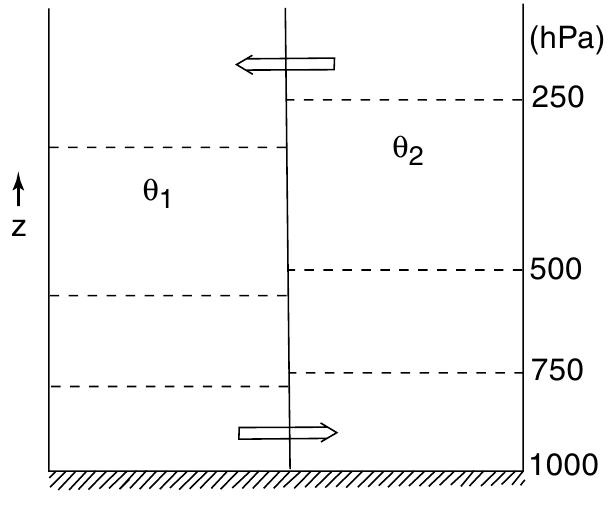
\includegraphics[scale=0.5]{{./chapters/figures_misc/holton_ape_fig}.jpeg}
\end{center}
\caption{Две воздушные массы с вертикальным разделителем. Пунктирные линии обозначают изобарические поверхности. Стрелки показывают направление движения, возникающего при удалении разделителя \citep{Holton2004}}
\label{fig:apeholton}
\end{figure}

Разность между полной потенциальной энергией и минимумом полной потенциальной энергии закрытой системы называется доступной потенциальной энергией (ДПЭ) и обозначается буквой $A$. Иначе говоря, ДПЭ есть разность между полной потенциальной энергией данного состояния атмосферы и потенциальной энергией фонового состояния. В отличие от кинетической или внутренней энергии, доступная потенциальная энергия есть интегральная характеристика и, согласно Лоренцу, пропорциональна квадрату отклонения потенциальной температуры от фонового состояния и обратно пропорциональна статической устойчивости. 

Наблюдения показывают, что лишь $0.5\%$ полной потенциальной энергии атмосферы доступно для перехода в другие виды энергии, и обычно только $10\%$ от этого количества преобразуется в кинетическую \citep{Holton2004}. С этой точки зрения атмосфера Земли является очень неэффективной тепловой машиной. 

Заметим, что перемещение масс в рассмотренном выше примере было адиабатическим. Следовательно, вывод точного выражения для ДПЭ удобно производить в изэнтропических координатах ($x,y,\theta$). При этом используем выражение для потенциальной энергии, проинтегрированное по всему расчетному объему. В данном разделе под $S$ понимается площадь, по которой производится интегрирование. Сначала запишем потенциальную энергию в изобарических координатах:
\begin{equation}
E_P=\frac{R}{g}\int_0^{p_0}dp
\end{equation}
а внутреннюю также представим через интеграл по давлению:
\begin{equation}
E_I=\frac{c_v}{g}\int_0^{p_0}Tdp
\end{equation}
Тогда полная потенциальная энергия (суммарная не только по высоте, но и по площади) будет равняться
\begin{equation}
E_T=\frac{c_p}{g}\iint_S\int_0^{p_0}TdpdS' = \frac{c_p}{g}\iint_S\int_0^{p_0}\theta\left(\frac{p}{p_{00}}\right)^\kappa dpdS' = \frac{c_p}{gp_{00}^\kappa (\kappa+1)}\iint_S\int_0^{p_0}\theta dp^{\kappa+1}dS'
\end{equation}
Это выражение путем некоторых преобразований с использованием правила интегрирования по частям и граничных условий на верхней и нижней границе атмосферы можно привести к виду
\begin{equation}
E_T=\frac{c_p}{gp_{00}^\kappa (\kappa+1)}\iint_S\int_0^{\infty}p^{\kappa+1}d\theta dS'
\end{equation}
Баротропное состояние характеризуется полной потенциальной энергией (с индексом $s$):
\begin{equation}
E_{T,s}=\frac{c_p}{gp_{00}^\kappa (\kappa+1)}\iint_S\int_0^{\infty}p_s^{\kappa+1}d\theta dS'
\end{equation}
Исходя из определения, доступная потенциальная энергия равна разности последних интегралов:
\begin{equation}
A=\frac{c_p}{gp_{00}^\kappa (\kappa+1)}\iint_S\int_0^{\infty}\left(p^{\kappa+1} - p_s^{\kappa+1}\right)d\theta dS'
\end{equation}
Пусть для давления p справедливо приближение Буссинеска
\begin{equation}
p=p_s+p', \quad p'/p_s \ll 1
\end{equation}
Тогда, если разложить подынтегральную часть выражения в степенной ряд и ограничиться двумя первыми членами разложения (причем первый из них после интегрирования исчезает), то
\begin{equation}
A=\frac{1}{2}\frac{\kappa c_p}{gp_{00}^\kappa}\iint_S\int_0^{\infty}p_s^{\kappa+1}\left(\frac{p'}{p_s}\right)^2 d\theta dS'
\end{equation}
Далее необходимо перейти обратно в изобарические координаты. Для этого принимаем
\begin{equation}
\theta - \hat{\theta}=\theta'=-\pderiv{\hat{\theta}}{p}p',
\end{equation}
что означает, что отклонение потенциальной температуры от среднего значения на изобарической поверхности пропорционально отклонению давления от его среднего на изотермической поверхности. 
Преобразовав дифференциал по формуле $d\theta=\pderiv{\theta}{p}dp$, получаем
\begin{equation}
A=-\frac{1}{2}\frac{R}{gp_{00}^\kappa}\iint_S\int_0^{p_0}p_s^{\kappa-1}\theta'^2\left(\pderiv{\hat{\theta}}{p}\right)^{-2}\pderiv{\theta}{p} dp dS'
\end{equation}
которое при равенстве $p=p_s$ на изобарической поверхности и при $\pderiv{\hat{\theta}}{p}\approx \pderiv{\theta}{p}$ преобразуется в окончательное выражение
\begin{equation} \label{eq:apeclassic}
A=-\frac{1}{2}\frac{R}{gp_{00}^\kappa}\iint_S\int_0^{p_0}p_s^{\kappa-1}\theta'^2\left(\pderiv{\hat{\theta}}{p}\right)^{-1} dp dS'
\end{equation}

\subsection{Кинетическая и доступная потенциальная энергия в уравнениях модели}
\label{sec:energymodel}
Отметим, что классическое выражение для ДПЭ \eqref{eq:apeclassic} не обязано выполняться для системы уравнений модели, которая получена при упрощениях исходной системы гидротермодинамики в z-координатах (Miranda, 1991). Поэтому ниже мы получим выражение ДПЭ, справедливое именно для модели ReMeDy, чтобы с помощью него корректно диагностировать ее результаты. Рассмотрим систему уравнений модели \eqref{eq:progn0}. Уравнения движения для трех компонент вектора скорости и уравнение притока тепла можно переписать, учитывая уравнение неразрывности \eqref{eq:progn5}, через полную производную в $\sigma$-координатах:
\begin{subequations}\label{eq:totderiv0}
\begin{align}
p_*\frac{Du}{Dt}&=-p_* \frac{\partial{\phi'}}{\partial{x}}+\sigma \frac{\partial{p_*}}{\partial{x}}\frac{\partial{\phi'}}{\partial{\sigma}}+f(v-V_g )p_*+p_*(D_u+R_u )\label{eq:totderiv1} \\
p_*\frac{Dv}{Dt}&=-p_* \frac{\partial{\phi'}}{\partial{y}}+\sigma \frac{\partial{p_*}}{\partial{y}}\frac{\partial{\phi'}}{\partial{\sigma}}-f(u-U_g )p_*+p_*(D_v+R_v )\label{eq:totderiv2} \\
p_*\frac{D\tilde{w}}{Dt}&=S_vp_* \frac{\partial{\phi'}}{\partial{\sigma}}+p_*g\frac{\theta'}{\theta_S}+p_*(D_{\tilde{w}}+R_{\tilde{w}})\label{eq:totderiv3} \\
p_*\frac{D\theta'}{Dt}&=S_v\tilde{w}p_*\frac{\partial{\theta_s}}{\partial{\sigma}}+p_*Q+p_*(D_{\theta}+R_{\theta}),\label{eq:totderiv4} 
\end{align}
\end{subequations}
где $\frac{D}{Dt}=\frac{\partial}{\partial{t}} +u \frac{\partial}{\partial{x}}+ v\frac{\partial}{\partial{y}}+ \dot{\sigma}\frac{\partial}{\partial{\sigma}}$.

\subsection{Бюджет полной кинетической энергии}
Известно, что удельная кинетическая энергия частицы $E_k$ пропорциональна сумме квадратов скорости:
$$E_k=\frac{1}{2}\left(u^2+v^2+\tilde{w}^2\right).$$
Уравнение для эволюции кинетической энергии получим, умножив каждое уравнение движения \eqref{eq:totderiv1}--\eqref{eq:totderiv3} на соответствующую компоненту вектора скорости и сложив полученные выражения:
\begin{subequations}\label{eq:ek0}
\begin{align}
\frac{1}{2}p_*\frac{Du^2}{Dt}&=-p_*u \frac{\partial{\phi'}}{\partial{x}}+\sigma u \frac{\partial{p_*}}{\partial{x}}\frac{\partial{\phi'}}{\partial{\sigma}}+f(v-V_g )p_*u+p_*u(D_u+R_u )\label{eq:ek1} \\
\frac{1}{2}p_*\frac{Dv^2}{Dt}&=-p_*v \frac{\partial{\phi'}}{\partial{y}}+\sigma v \frac{\partial{p_*}}{\partial{y}}\frac{\partial{\phi'}}{\partial{\sigma}}-f(u-U_g )p_*v+p_*v(D_v+R_v )\label{eq:ek2} \\
\frac{1}{2}p_*\frac{D\tilde{w}^2}{Dt}&=S_vp_*\tilde{w}\frac{\partial{\phi'}}{\partial{\sigma}}+p_*g\tilde{w}\frac{\theta'}{\theta_S}+p_*\tilde{w}(D_{\tilde{w}}+R_{\tilde{w}})\label{eq:ek3} \\
p_*\frac{DE_k}{Dt}&=-p_*u \pderiv{\phi'}{x}-p_*v \pderiv{\phi'}{y}+\sigma u \pderiv{p_*}{x}\pderiv{\phi'}{\sigma}+\sigma v \pderiv{p_*}{y}\pderiv{\phi'}{\sigma}+S_vp_*\tilde{w}\pderiv{\phi'}{\sigma}+\nonumber \\ 
&+p_*g\tilde{w}\frac{\theta'}{\theta_S}+fp_*(vU_g-uV_g) + \mathcal{D}_{u,v,w}, \label{eq:ek4}
\end{align}
\end{subequations}
где $\mathcal{D}_{u,v,w}$ обозначает сумму слагаемых, ответственных за турбулентную вязкость, пространственные и временные фильтры, приводящие к диссипации КЭ.

Первые пять слагаемых в правой части \eqref{eq:ek4} могут быть переписаны в более удобной форме (компоненты геострофической скорости опущены):
\begin{align}
 &-p_*u \pderiv{\phi'}{x}-p_*v \pderiv{\phi'}{y}+\sigma u \pderiv{p_*}{x}\pderiv{\phi'}{\sigma}+\sigma v \pderiv{p_*}{y}\pderiv{\phi'}{\sigma}+S_vp_*\tilde{w}\pderiv{\phi'}{\sigma}= \nonumber \\
=&-p_*u \pderiv{\phi'}{x}-p_*v \pderiv{\phi'}{y}+\sigma\pderiv{\phi'}{\sigma}\left(u\pderiv{p_*}{x}+ v\pderiv{p_*}{y}\right)-(p_*\dot{\sigma}+\sigma\dot{p_*})\pderiv{\phi'}{\sigma}= \nonumber \\
=&-p_*u \pderiv{\phi'}{x}-p_*v \pderiv{\phi'}{y}+\sigma\pderiv{\phi'}{\sigma}\left(u\pderiv{p_*}{x}+v\pderiv{p_*}{y}\right)-\sigma\pderiv{\phi'}{\sigma}\frac{Dp_*}{Dt}-p_*\dot{\sigma}\pderiv{\phi'}{\sigma}=\nonumber\\
=&-p_*u \pderiv{\phi'}{x}-p_*v \pderiv{\phi'}{y}-\sigma\pderiv{\phi'}{\sigma}\pderiv{p_*}{t}-p_*\dot{\sigma}\pderiv{\phi'}{\sigma}=\nonumber\\
=&-p_*u \pderiv{\phi'}{x}-p_*v \pderiv{\phi'}{y}-\phi'\left(u\pderiv{p_*}{x}+v\pderiv{p_*}{y}\right)-p_*\dot{\sigma}\pderiv{\phi'}{\sigma}+\phi'\left(u\pderiv{p_*}{x}+v\pderiv{p_*}{y}\right)+\phi'\pderiv{p_*}{t}-\phi'\pderiv{p_*}{t}-\sigma\pderiv{\phi'}{\sigma}\pderiv{p_*}{t}=\nonumber\\
=&-p_*u \pderiv{\phi'}{x}-p_*v \pderiv{\phi'}{y}-\phi'\left(u\pderiv{p_*}{x}+v\pderiv{p_*}{y}\right)-p_*\dot{\sigma}\pderiv{\phi'}{\sigma}+\phi'\frac{Dp_*}{Dt}-\phi'\pderiv{p_*}{t}-\sigma\pderiv{\phi'}{\sigma}\pderiv{p_*}{t}=\nonumber\\
=&-u \pderiv{p_*\phi'}{x}-v \pderiv{p_*\phi'}{y}-p_*\dot{\sigma}\pderiv{\phi'}{\sigma}+\phi'\frac{Dp_*}{Dt}-\pderiv{p_*}{t}\pderiv{(\sigma\phi')}{\sigma}=\nonumber\\
=&-u \pderiv{p_*\phi'}{x}-v \pderiv{p_*\phi'}{y}-\dot{\sigma}\pderiv{p_*\phi'}{\sigma}-\phi'p_*\left(\pderiv{u}{x}+\pderiv{v}{y}+\pderiv{\dot{\sigma}}{\sigma}\right)-\pderiv{p_*}{t}\pderiv{(\sigma\phi')}{\sigma}=\nonumber\\
=&-\pderiv{p_*u\phi'}{x}-\pderiv{p_*v\phi'}{y}-\pderiv{p_*\dot{\sigma}\phi'}{\sigma}-\pderiv{p_*}{t}\pderiv{(\sigma\phi')}{\sigma}.
\end{align}

После этих преобразований выражение для кинетической энергии можно переписать в дивергентной форме:
\begin{subequations}
\begin{align}
p_*\frac{DE_k}{Dt}&=-\pderiv{p_*u\phi'}{x}-\pderiv{p_*v\phi'}{y}-\pderiv{p_*\dot{\sigma}\phi'}{\sigma}-\pderiv{p_*}{t}\pderiv{\sigma\phi'}{\sigma}+p_*g\tilde{w}\frac{\theta'}{\theta_S}-fp_*(V_gu-U_gv) + \mathcal{D}_{u,v,w}, \\
\intertext{или} \nonumber \\
\frac{\partial{p_*E_k}}{\partial{t}}&=-\frac{\partial{p_*uE_k}}{\partial{x}}-\frac{\partial{p_*vE_k}}{\partial{y}}-\frac{\partial{p_*\dot{\sigma}E_k}}{\partial{\sigma}}-\frac{\partial{p_*u\phi'}}{\partial{x}}-\frac{\partial{p_*v\phi'}}{\partial{y}}-\frac{\partial{p_*\dot{\sigma}\phi'}}{\partial{\sigma}}+ \nonumber \\ 
&-\pderiv{p_*}{t}\pderiv{\sigma\phi'}{\sigma}+p_*g\tilde{w}\frac{\theta'}{\theta_S}-fp_*(V_gu-U_gv) + \mathcal{D}_{u,v,w} \label{eq:ektend}.
\end{align}
\end{subequations}

\subsection{Бюджет доступной энергии}
Чтобы получить аналогичное уравнение для доступной потенциальной энергии (ДПЭ), сначала умножим уравнение \eqref{eq:totderiv4} на возмущение потенциальной температуры $\theta'$:
\begin{align}
\frac{1}{2}p_*\frac{D\theta'^2}{Dt}&=S_v\tilde{w}p_*\theta'\frac{\partial{\theta_s}}{\partial{\sigma}}+p_*\theta'Q+p_*\theta'(D_{\theta}+R_{\theta}) \label{eq:th2}.
\end{align}

Как было показано в предыдущем разделе, ДПЭ пропорциональна квадрату отклонения потенциальной температуры от фонового состояния, деленной на статическую устойчивость. В системе координат модели ReMeDy статическая устойчивость, или квадрат частоты Брента-Вяйсяля, записывается следующим образом 
\begin{equation}
N^2=-S_v\frac{g}{\theta_s}\frac{\partial\theta_s}{\partial\sigma}. \label{eq:bfreq}
\end{equation}

Тогда разделим \eqref{eq:th2} на $N^2$ и умножим его на $\left(\frac{g}{\theta_s}\right)^2$. Другими словами, умножим уравнение притока тепла на величину, обратную градиенту температуры, обозначив ее $B^2$:
\begin{subequations}
\begin{align}
\frac{1}{2}p_*B^2\frac{D\theta'^2}{Dt}&=-gp_*\tilde{w}\frac{\theta'}{\theta_s}+p_*\theta'B^2Q+p_*\theta'B^2(D_{\theta}+R_{\theta})
\intertext{где}
B^2&=\left(\frac{g}{\theta_s}\right)^2N^{-2}=-\frac{g/\theta_s}{S_v \partial\theta_s/\partial\sigma}=\frac{g/\theta_s}{ \partial\theta_s/\partial{z}} \label{eq:B2}.
\end{align}
\end{subequations}

Используя правило дифференцирования произведения и уравнение неразрывности \eqref{eq:progn5}, можно записать
\begin{align}
\frac{1}{2}p_*\frac{D\theta'^2B^2}{Dt}&=\frac{1}{2}\left(\frac{\partial{p_*\theta'^2B^2}}{\partial{t}}+\frac{\partial{p_*u\theta'^2B^2}}{\partial{x}}+\frac{\partial{p_*v\theta'^2B^2}}{\partial{y}}+\frac{\partial{p_*\dot{\sigma}\theta'^2B^2}}{\partial{\sigma}}\right)= \nonumber\\ 
&=-gp_*\tilde{w}\frac{\theta'}{\theta_s}+\frac{1}{2}p_*\theta'^2\frac{DB^2}{Dt}+p_*\theta'B^2Q+p_*\theta'B^2(\mathcal{D}_{\theta}+R_{\theta}) \label{eq:apetend}
\end{align}
где $\theta'^2B^2$ может быть интерпретировано как ДПЭ на единицу массы. Под знаком полной производной находится выражение, которое есть доступная потенциальная энергия. Если сравнить \eqref{eq:ektend} и \eqref{eq:apetend2}, становится видно, что слагаемое $gp_*\tilde{w}\frac{\theta'}{\theta_s}$, которое присутствует в обоих уравнениях, но с разными знаками, можно интерпретировать как переход энергии из доступной потенциальной в кинетическую и обратно.

Согласно \eqref{eq:B2}, параметр $B^2$ зависит только от вертикальной координаты. Следовательно, полная производная, входящая во второе слагаемое в правой части уравнения \eqref{eq:apetend}, после нескольких преобразований превращается в следующее выражение
\begin{align}
\frac{DB^2}{Dt}=\frac{\partial{B^2}}{\partial{t}}+u \frac{\partial{B^2}}{\partial{x}}+v\frac{\partial{B^2}}{\partial{y}}+\tilde{w}\frac{\partial{B^2}}{\partial{z}} \approx \tilde{w}\frac{\partial{B^2}}{\partial{z}}=-\frac{g\tilde{w}}{\theta_s}\left(\frac{\partial\theta_s}{\partial{z}}\right)^{-2}\left(\frac{Dln\theta_s}{Dz}-\frac{D^2\theta_s}{Dz^2}\right) \label{eq:dB2}.
\end{align}
Отметим, что если фоновое изменение потенциальной температуры задано линейной функцией, то вычитаемое, стоящее в скобках \eqref{eq:dB2}, становится равным нулю. В данной работе профиль $\theta_s$ являлся именно линейным, так что 
\begin{equation}
B^2=-\frac{g\tilde{w}}{\theta_s^2}\left(\frac{\partial\theta_s}{\partial{z}}\right)^{-1}
\end{equation}
Значит, тенденцию ДПЭ на единицу массы, $E_a=\frac{1}{2}\theta'^2B^2$, можно переписать в виде
\begin{align}
\frac{\partial p_*E_a}{\partial{t}}&=-\frac{\partial{p_*uE_a}}{\partial{x}}-\frac{\partial{p_*vE_a}}{\partial{y}}-\frac{\partial{p_*\dot{\sigma}E_a}}{\partial{\sigma}} \nonumber\\ 
&=-gp_*\tilde{w}\frac{\theta'}{\theta_s}-\frac{1}{2}gp_*\tilde{w}\left(\frac{\theta'}{\theta_s}\right)^2\left(\frac{\partial\theta_s}{\partial{z}}\right)^{-1}p_*\theta'B^2(Q+\mathcal{D}_\theta) \label{eq:apetend2}.
\end{align} %%+gp_*\frac{\theta'}{\theta_s}\frac{1}{ \partial\theta_s/\partial{z}}\frac{L_v}{c_p}\left(\frac{p_0}{p}\right)^{R_d/c_p}(C-E)

Доступная потенциальная энергия, как было показано в разделе \ref{sec:APEtheory}, есть интегральная величина. Принимая во внимание верхнее и нижнее граничные условия ($\dot{\sigma}_{\sigma=0,1}=0$), получаем интегральную форму уравнений \eqref{eq:apetend2} и \eqref{eq:ektend}. Так, изменение полной (интегральной) кинетической энергии $K=\frac{1}{g}\iiint\limits_V p_*E_k dxdyd\sigma$ во времени равно:
\begin{align} \label{eq:dKdt}
\frac{d}{dt}K&=\frac{1}{g}\iint\left[(p_*uE_k)_{x=x_1}-(p_*uE_k)_{x=x_2}\right]dyd\sigma + \frac{1}{g}\iint\left[(p_*vE_k)_{y=y_1}-(p_*vE_k)_{y=y_2}\right]dxd\sigma + \nonumber\\ &+\frac{1}{g}\iint\left[(p_*u\phi^\prime)_{x=x_1}-(p_*u\phi^\prime)_{x=x_2}\right]dyd\sigma + \frac{1}{g}\iint\left[(p_*v\phi^\prime)_{y=y_1}-(p_*v\phi^\prime)_{y=y_2}\right] dxd\sigma + \nonumber\\ &+ \iiint p_*\tilde{w}\frac{\theta^\prime}{\theta_s}dxdyd\sigma - \frac{1}{g}\iiint p_*f(V_gu-U_gv) dxdyd\sigma+\frac{1}{g}\iiint \mathcal{D}_{u,v,w}dxdyd\sigma
\end{align}
а изменение ДПЭ, $A=\frac{1}{g}\iiint\limits_V p_*E_a dxdyd\sigma$ равно:
\begin{align} \label{eq:dAdt}
\frac{d}{dt}A&=\frac{1}{g}\iint\left[(p_*uE_a)_{x=x_1}-(p_*uE_a)_{x=x_2}\right]dyd\sigma + \frac{1}{g}\iint\left[(p_*vE_a)_{y=y_1}-(p_*vE_a)_{y=y_2}\right]dxd\sigma - \nonumber\\ &- \iiint p_*\tilde{w}\frac{\theta^\prime}{\theta_s}dxdyd\sigma \nonumber\\
&+ \frac{1}{2}\iiint p_*\tilde{w}\left(\frac{\theta^\prime}{\theta_s}\right)^2\left(\frac{\partial\theta_s}{\partial z}\right)^{-1}dxdyd\sigma+\frac{1}{g}\iiint p_*\theta'B^2Qdxdyd\sigma+\frac{1}{g}\iiint p_*\theta'B^2\mathcal{D}_{\theta}dxdyd\sigma.
\end{align} %+\iiint \left(p_*\frac{\theta'}{\theta_s}\frac{1}{ \partial\theta_s/\partial{z}}\frac{L_v}{c_p}\left(\frac{p_0}{p}\right)^{R_d/c_p}(C-E)\right) dxdyd\sigma

\subsubsection{Потоки тепла с поверхности}
\label{sec:expsetup:hsurf}
Вернемся к выражению \eqref{eq:apetend}. Заметим, что первое слагаемое в скобках отвечает за подсеточное турбулентное перемешивание, и в модели определяется через коэффициент турбулентной теплопроводности (для замыкания Смагоринского-Лилли, см. раздел \ref{sec:model:closure}.

Термическая диффузия в нашей работе представлялась только вертикальной ее компонентой, так что для простоты следующие выкладки будут включать пространственные производные только для $\sigma$:
\begin{equation}
D_\theta=S_v\pderiv{}{\sigma}K_H S_v\pderiv{\theta}{\sigma}
\end{equation}

Интегрирование этого выражения по высоте и использование правила интегрирования по частям дает
\begin{align}
\int_\sigma p_*\theta'B^2S_v\pderiv{}{\sigma}\left(K_H S_v\pderiv{\theta}{\sigma}\right)d\sigma&=\left(p_*\theta'B^2S_v^2K_H \pderiv{\theta}{\sigma}\right)_{\sigma=0}-\left(p_*\theta'B^2S_v^2K_H \pderiv{\theta}{\sigma}\right)_{\sigma=1} \\ 
&-\int_\sigma p_*\pderiv{\theta'S_vB^2}{\sigma}S_vK_H\pderiv{\theta}{\sigma}d\sigma \label{eq:subgrid_mixing_theta}
\end{align}
Первое слагаемое в правой части уравнения выше включает поток тепла на верхней границе области, который в силу граничных условий равен нулю, в то время как второе слагаемое определяется нижним граничным условием, которое зависит от потока тепла с поверхности ($H_{surf}=-K_H S_v\pderiv{\theta}{\sigma}c_p\rho\left(\frac{p}{p_0}\right)^{\kappa}$). Последний член в \eqref{eq:subgrid_mixing_theta} может быть интерпретирован как диссипация ДПЭ через теплопроводность. В результате этих преобразований ур. \eqref{eq:subgrid_mixing_theta} принимает вид:
\begin{equation}
\int_\sigma\theta'B^2\mathcal{D}_\theta d\sigma=\left(\theta'B^2S_v\right)_{\sigma=1}\frac{H_{surf}}{c_p\rho}\left(\frac{p_0}{p}\right)^{\kappa}-\int_\sigma \pderiv{\theta'S_vB^2}{\sigma}S_vK_H\pderiv{\theta}{\sigma}d\sigma \label{eq:subgrid_mixing_theta_fin}
\end{equation}

\begin{thebibliography}{12}
 \bibitem{ER89}
Emanuel KA, Rotunno R. 1989. Polar lows as Arctic hurricanes. \textit{Tellus} \textbf{41A:} 1-17.
\end{thebibliography}

\end{document}